\chapter{Three-Operand Binary Adder Techniques}

The three-operands binary addition is one of the critical arithmetic operation in the congruential modular arithmetic architectures [5] – [8] and LCG-based PRBG methods such as CLCG [9], MDCLCG [10] and CVLCG [11]. It can be implemented either by using two stages of two-operands adders or one stage of three-operand adder.

\section{Three operands Carry Save Adder}
Carry-save adder (CSA) is the commonly used technique to perform the three-operand binary addition [9]–[14]. It computes the addition of three operands in two stages. The first stage is the array of full adders. Each full adder computes “carry” bit and “sum” bit concurrently from three binary input $ a_{i} $ , $ b_{i} $ and $ c_{i} $ . The second stage is the ripple-carry adder that computes the final n-bit size “sum” and one-bit size “carry-out” signals at the output of three-operand addition. The “carry-out” signal is propagated through the n number of full adders in the ripple-carry stage. Therefore, the delay increases linearly with the increase of bit length. The architecture of the three-operand carry-save adder is shown in Fig.~\ref{fig:x3} and the critical path delay is highlighted with a dashed line. It shows that the critical path delay depends on the carry propagation delay of ripple carry stage and is evaluated as follows,
\begin{equation}
 T_{CS3A} = (n+1)T_{FA} = 3T_{X} + 2_{n}T_{G}
 \label{eq1} 
\end{equation}
Similarly, the total area is evaluated as follows,
\begin{equation}
A_{CS3A} = 2nA_{FA} = 4nA_{X} + 6nA_{G}
	\label{eq2}
\end{equation}
Here, $ A_{G} $ and $ T_{G} $ indicate the area and propagation delay of basic 2-input gate (AND/OR/NAND/NOR) respectively. $ A_{X} $ and $ T_{X} $ indicate the area and propagation delay of 2-input XOR gate respectively. The major drawback of the CS3A is the larger critical path delay which increases with an increase of bit length. This critical propagation path delay influences the overall latency of the congruential modular arithmetic based cryptography and PRBG architectures, where three-operand adder is the primary component.
\begin{figure}[htb]
	\centering
	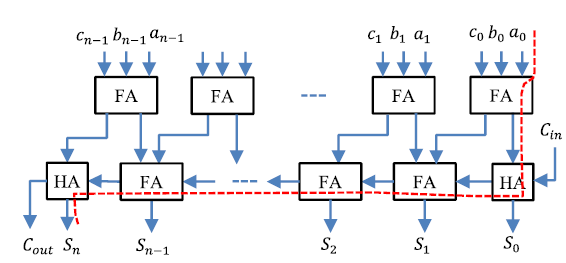
\includegraphics[width=0.80\columnwidth]{Figures/x3}	
	\caption{Three-operands carry-save adder (CS3A)}
	\label{fig:x3}
\end{figure}


\section{High-Speed Area Efficient Three Operands Adder}
This section presents a new adder technique and its VLSI architecture to perform the three-operand addition in modular arithmetic. The  adder technique is a parallel prefix adder.
\subsection{Overview of HSAE Adder}
The HSAE adder has four-stage structures instead three-stage structures in prefix adder to compute the addition of three binary input operands such as bit-addition logic, base logic, PG (propagate and generate) logic and sum logic. The logical expression of all these four stages is defined as follows,
\begin{figure}[htb]
	\centering
	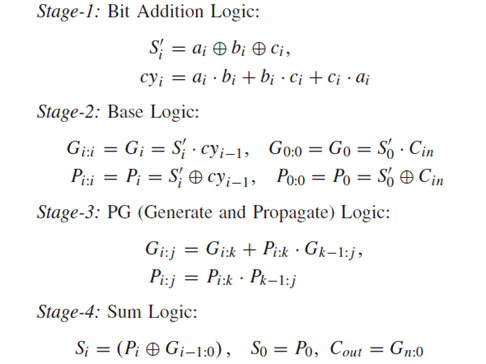
\includegraphics[width=0.80\columnwidth]{Figures/x4}	
%	\caption{Three-operands carry-save adder (CS3A)}
	\label{fig:x4}
\end{figure}
The proposed VLSI architecture of the three-operand binary adder and its internal structure is shown in Fig.~\ref{fig:x5}. The new adder technique performs the addition of three n-bit binary inputs in four different stages. In the first stage (bit-addition logic), the bitwise addition of three n-bit binary input operands is performed with the array of full adders, and each full adder computes “sum ($ S'_{i} $)” and “carry ($ cy_{i} $)” signals as highlighted in Fig.~\ref{fig:x5} (a). The logical expressions for computing sum ($ S'_{i} $) and carry ($ cy_{i} $ ) signals are defined in Stage-1, and the logical diagram of the bit-addition logic is shown in Fig.~\ref*{fig:x5} (b). \par 
In the first stage, the output signal “sum ($ S'_{i} $)” bit of current full adder and the output signal “carry” bit of its right-adjacent full adder are used together to compute the generate ($ G_{i} $) and propagate ($ P_{i} $) signals in the second stage (base logic). The computation of $ G_{i} $ and $ P_{i} $ signals are represented by the “squared saltire-cell” as shown in Fig.~\ref{fig:x5} (a) and there is n+1 number of saltire-cells in the base logic stage. The logic diagram of the saltire-cell is shown in Fig.~\ref{fig:x5} (b), and it is realized by the following logical expression,
\begin{equation}
G_{i:i} = G_{i} = S'_{i} \cdot cy_{i−1}
	\label{eq3}
\end{equation}
\begin{equation}
P_{i:i} = P_{i} = S'_{i} \cdot cy_{i−1}
	\label{eq4}
\end{equation}
The external carry-input signal ($ C_{in} $) is also taken into consideration for three-operand addition in the proposed adder technique. This additional carry-input signal ($ C_{in} $) is taken as input to base logic while computing the $ G_{0}(S'_{0} \cdot C_{in}) $ in the first saltire-cell of the base logic.
\begin{figure}[htb]
	\centering
	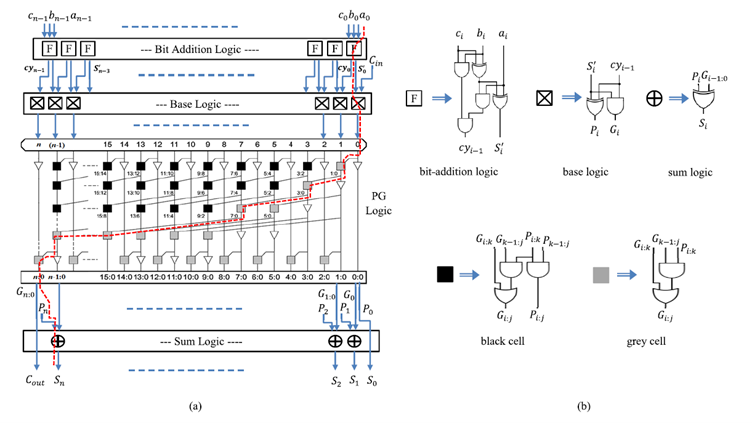
\includegraphics[width=0.80\columnwidth]{Figures/x5}	
	\caption{High Speed Area Efficient Adder}
	\label{fig:x5}
\end{figure}
The third stage is the carry computation stage called “generate and propagate logic” (PG) to pre-compute the carry bit and is the combination of black and grey cell logics. The logical diagram of black and grey cell is shown in Fig.~\ref{fig:x5} (b) that computes the carry generate $ G_{i:j} $ and propagate $ P_{i:j} $ signals with the following logical expression,
\begin{equation}
G_{i:j} = G_{i:k} + P_{i:k} \cdot G_{k−1:j}
	\label{eq5}
\end{equation}
\begin{equation}
P_{i:j} = P_{i:k} \cdot P_{k−1:j}
	\label{eq6}
\end{equation}
The number of prefix computation stages for the proposed adder is $(\log_{2}n + 1)$ , and therefore, the critical path delay of the proposed adder is mainly influenced by this carry propagate chain. \par
The final stage is represented as sum logic in which the “sum ($ S_{i} $)” bits are computed from the carry generate $ G_{i:j} $ and carry propagate $ P_{i} $ bits using the logical expression, $ S_{i} = (P_{i} \oplus G_{i−1:0}) $. The carryout signal ($ C_{out} $) is directly obtained from the carry generate bit $ G_{n:0} $.








